\beginsong{Abend ward}[wuw={Rudolf Alexander Schröder, Friedrich Samuel Rothenberg, 1942}, bo={4}, pfiii={73}, gruen={110}, kssiv={6}]

\beginverse
\endverse
\centering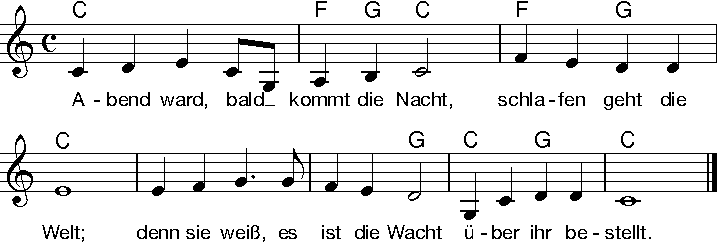
\includegraphics[width=1\textwidth]{Noten/Lied001.pdf}	

\beginverse
\[C]Einer wacht und \[F]trägt \[G]all\[C]ein
\[F]ihre \[G]Müh' und \[C]Plag',
der lässt keinen einsam \[G]sein, 
\[C]weder \[G]Nacht noch \[C]Tag.
\endverse 

\beginverse
^Jesus Christ, mein ^Hort ^und ^Halt,
^dein ge^denk' ich ^nun,
tu mit Bitten dir Ge^walt, 
^bleib bei ^meinem ^Ruhm.
\endverse

\beginverse
^Wenn Dein Aug' ob ^mei^nem ^wacht,
^wenn Dein ^Trost mir ^frommt,
weiß ich, dass auf gute ^Nacht 
^guter ^Morgen ^kommt.
\endverse

\endsong
